\section{Software Implementation}
In the following section, the actual software implementation of the system will be covered. The image processing algorithm that was developed in Bjørnsen 2016\cite{kris} is further developed and ported from MATLAB to Python. Other than the image processing algorithm, the communication between the Raspberry Pi and a computer, as well as the camera and image capturing is also presented. \\

The implementation is built up as follows:
\begin{enumerate}
\item Image capture by camera with scaling
\item Image processing. Consisting of:
\begin{enumerate}
\item Edge detection using the Canny algorithm
\item Hough transform to identify wall segments
\end{enumerate}
\item Mapping. Consisting of:
\begin{enumerate}
\item Range sensor implementation
\item Transformation from pixel coordinates to real life coordinates using GSD
\end{enumerate}
\item Communication:
\begin{enumerate}
\item SSH
\item Protocol and format
\end{enumerate}
\end{enumerate}


\subsection{Camera and Image Capturing}
Our system should be able to capture an image with the camera and store it in memory so that the image processing algorithm can be run with it. By using the PiCamera\cite{picam} framework, I am able to call functions in Python that will capture and save the image, as well as defining variables and operations relating to the image.\\

To be able to use the module I must import PiCamera in the beginning of the sofware:

\begin{minted}[frame=single,framesep=2pt,linenos]{python}
from picamera import PiCamera
\end{minted}
I designed the capture function such that it returns the captured image, and is designed to be run from the main loop function. The resolution of the image can be changed by setting the \texttt{camera.resolution}. The maximum resolution for the Raspberry Pi camera is $3280\times2464$.

\begin{minted}[frame=single,framesep=2pt,linenos]{python}
def capture():
    #Initialize camera
    camera = PiCamera()
    #Set camera resolution
    camera.resolution = (3280,2464)
    #Capture image and save
    camera.capture('Image.png')
    #Open image in greyscale
    I = cv2.imread('Image.png',0)
    #Resize image
    I = cv2.resize(I, (0,0), fx=0.4, fy=0.4)
    #Return image I
    return I
\end{minted}
This is the most basic implementation of camera capture, and most of the technical aspects such as focus and light correction is done in the \texttt{camera.capture} function.


\subsection{Image Processing}
The image processing part of the software is similar to that found in Bjørnsen 2016\cite{kris}, only that it is programmed in Python. Some of the MATLAB functionality found in the Image Processing Toolbox are not the same as that of the OpenCV library, but yields similar results. \\

The image processing section uses OpenCV and Numpy for the calculations. They must be included in the beginning:

\begin{minted}[frame=single,framesep=2pt,linenos]{python}
import numpy as np
import cv2
\end{minted}

The implementation is described below. It includes a part which draws the detected lines on the original picture. This is for testing purposes to see if I manage to detect the whole wall segment.
\begin{minted}[frame=single,framesep=2pt,linenos]{python}
def detectedges(img):
    #Canny edge detection
    threshold = 700
    BW2 = cv2.Canny(img,threshold,threshold*0.4)
    
    #Set minimum line length and line gap
    minLineLength = 300
    maxLineGap = 0

    #Hough Transform
    lines = cv2.HoughLinesP(BW2,1,np.pi/180,0,100,320,130)

    #Return to BGR so I can draw green lines on the image
    img = cv2.cvtColor(img, cv2.COLOR_GRAY2BGR)
    
    #Draw lines on picture
    for i in range(len(lines)):
        for x1,y1,x2,y2 in lines[i]:
            cv2.line(img,(x1,y1),(x2,y2),(0,255,0),4)
        cv2.imwrite('houghlines.jpg',img)

    #HoughLinesP saves a 3D array. convert to 2D array
    lines = lines.squeeze()
    
    return lines
\end{minted}

\subsubsection{Edge detection}
The edge detection part of the implementation is done on lines 3 and 4. The threshold value is a empirically tuned variable determined from the image. The maze we are going to map has a dark top side, which enables me to set the threshold value relatively high. Usually it ranges from 300 to 700. \\

For the actual edge detection I am using the Canny edge algorithm. This is implemented as \texttt{cv2.Canny(image,upper\_threshold,lower\_threshold)} in the OpenCV framework. This returns an array of detected edges, which can then be used in the Hough transform.

\begin{minted}[frame=single,framesep=2pt,linenos]{python}
    #Canny edge detection
    threshold = 700
    BW2 = cv2.Canny(img,threshold,threshold*0.4)
\end{minted}

\subsubsection{Hough Transform}
As explained in the theory part of the paper, the Hough transform is used to link the detected edges together into meaningful segments. In this application that means linking in such a way that we can represent the detected edges along a wall as an actual wall. This is done by setting the minimum line length and maximum line gap that it should fill, and running the \texttt{cv2.HoughLinesP(image, rho, theta, threshold[, lines[, minLineLength[, maxLineGap]]])} function. This is an implementation of the probabilistic Hough Transform that finds line segments.\\

The input variables for this function is tuned for the size of the line segments on the array of detected lines. The other input variables such as rho and theta can be recognized from the theory part.\\

The \texttt{cv2.HoughLinesP} function returns a 3D array, but what I really want is a 2D array. The reason it does this originates from the official translation of the code from C++ to Python. By running \texttt{squeeze()} on the array I delete the empty dimension of the array, and this can be returned.

\begin{minted}[frame=single,framesep=2pt,linenos]{python}
    #Set minimum line length and line gap
    minLineLength = 300
    maxLineGap = 130
    threshold = 0

    #Hough Transform
    lines = cv2.HoughLinesP(BW2,1,np.pi/180,threshold,100,
    			minLineLength,maxLineGap)
    
    #HoughLinesP saves a 3D array. convert to 2D array
    lines = lines.squeeze()
\end{minted}

\subsection{Range sensor implementation}
The range sensor is implemented in a \texttt{getdistance()} function which returns the detected range from the HC-SR04. The code was collected from ModMyPi\cite{prange} and modified.\\

The first part of the function defines the GPIO interface, that is, which pins are echo, and which is trig. By detecting the output of these pins, and measuring the time it takes, the distance can be calculated. In order for this function to work the following must be imported at the start of the program:

\begin{minted}[frame=single,framesep=2pt,linenos]{python}
import RPi.GPIO as GPIO
import time
GPIO.setmode(GPIO.BCM)
\end{minted}

\begin{minted}[frame=single,framesep=2pt,linenos]{python}
def getdistance():
    #Define GPIO pins on the Raspberry Pi
    TRIG = 18 
    ECHO = 24
    
    #Set which pins is echo and trig
    GPIO.setup(TRIG,GPIO.OUT)
    GPIO.setup(ECHO,GPIO.IN)
    GPIO.output(TRIG, False)
    
    #Sleep while sensor settles
    time.sleep(2)
    GPIO.output(TRIG, True)
    time.sleep(0.00001)
    GPIO.output(TRIG, False)

    #Get the time for the calculation
    while GPIO.input(ECHO)==0:
        pulse_start = time.time()
    while GPIO.input(ECHO)==1:
        pulse_end = time.time()

    #Calculate the distance
    pulse_duration = pulse_end - pulse_start
    distance = pulse_duration * 17150
    distance = round(distance, 2)
    
    return distance
\end{minted}
The theory behind the distance calculation is explained in Section \ref{urs}. 


\subsection{Mapping}
The mapping part of the implementation is implemented in the \texttt{mapping(lines, distance)} function. This function takes in the detected line segments from the Hough Transform, and the detected distance from the range sensor implementation, as well as the wall height. From this information it is able to transform the detected lines from pixel values to real life units.\\

The actual translation is done by multiplying the calculated GSD with each detected line segment, and updating the list. 

\begin{minted}[frame=single,framesep=2pt,linenos]{python}
def mapping(lines, distance,wall_h):
    ###Calculate GSD
    #Sensor width
    Sw = 3.68
    #Focal length
    Fr = 3.04
    #Height
    H = distance-wall_h
    #Image size
    Iw = 3280
    Ih = 2464
    #GSD in cm/pixel
    GSD = (Sw*H)/(Fr*Iw)
	
    #Apply to lines
    for i in range(len(lines)):
        lines[i] = GSD*lines[i]
        
    #Return scaled lines
    return lines
\end{minted}

\subsection{Main function}
The main function is based on the implementation presented in the beginning of this section. It does a step-by-step function call procedure that will yield the desired line segments of the walls detected. After this it will print the results to be collected on a SSH remote terminal.
\begin{minted}[frame=single,framesep=2pt,linenos,breaklines]{python}
def main():
    #Define wall heigth
    wall_h = 30
    
    #Capture image
    img = capture()
    #Detect lines
    lines = detectedges(img)
    #Get distance
    distance = getdistance()
    #Mapping 
    reallines = mapping(lines,distance,wall_h)

    #Positioning (not implemented; for communication)
    x = 0
    y = 0
    theta = 90

    for i in range(len(reallines)):
        print("{U: %s, %s, %s, %s, %s, %s, %s}" % (x, y, theta, reallines[i][0], reallines[i][1]
    	,reallines[i][2],reallines[i][3]))
        
    #Cleanup
    GPIO.cleanup()
\end{minted}

\subsection{Communication}
The communication with the Raspberry Pi and the software is meant for SSH in this implementation. The communication is achieved by connecting the Raspberry Pi remotely through SSH and running the program while reading the output on the master computer. \\

The SSH master computer is in this implementation running Windows (similar to the LEGO robot server), and to establish SSH with the Raspberry Pi, a SSH client must be downloaded. The program of choice for this is PuTTY \cite{putty}. By typing the local IP of the Raspberry Pi in the "Host Name", one can connect easily. 

\begin{figure}[H]
  \centering
  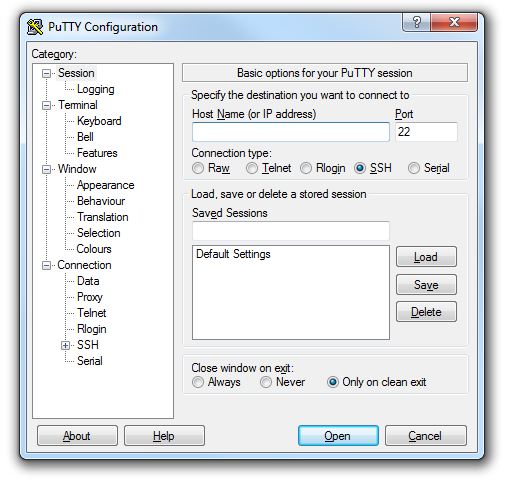
\includegraphics[width=0.6\textwidth]{fig/putty}
  \caption{PuTTY in Windows}
  \label{fig:putty}
\end{figure}

After typing the Raspberry Pi local IP, the following window will appear: 

\begin{figure}[H]
  \centering
  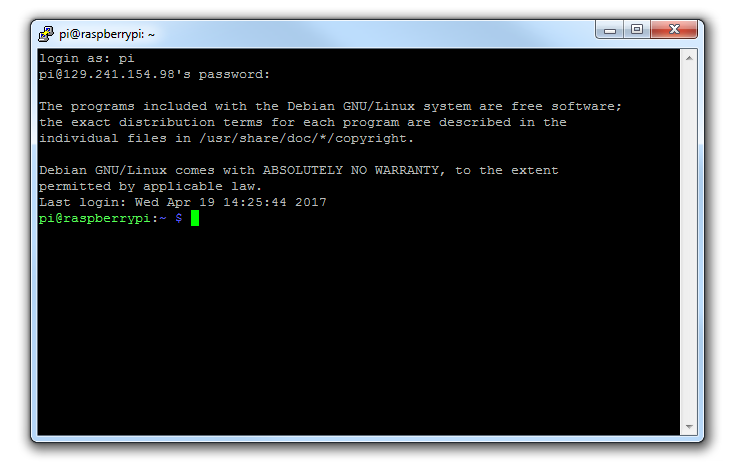
\includegraphics[width=0.7\textwidth]{fig/putty2}
  \caption{PuTTY terminal in Windows}
  \label{fig:putty}
\end{figure}
From here the program can be run remotely from the master computer. By running the program from there the output of the program will also be communicated over SSH in the terminal. 

\subsubsection{Protocol}
The implementation of the LEGO robots features a communication protocol to communicate various pieces of sensor data to the host. Some of the other Master students working on this have provided me with a communication protocol that my implementation can be built around to facilitate for better integration with the existing solution in the future. \\

The protocol is implemented in the main function mentioned previously, and it is built as follows:

\begin{table}[H]
\centering
\label{protocol}
\begin{tabular}{|l|l|l|l|l|l|l|l|}
\hline
\textbf{\{U:} & \textbf{X} & \textbf{Y} & \textbf{Theta} & \textbf{Line Start X} & \textbf{Line Start Y} & \textbf{Line Stop X} & \textbf{Line Stop Y\}} \\ \hline
\end{tabular}
\caption{Update message protocol}
\end{table}

The fields should be separated by commas, and initiated with \textbf{U:} to identify the message as an "Update" message in the LEGO communication protocol.XXXX. The whole message should be in curly brackets. \\

The first three fields after the message identifier \textbf{U:}, is the X,Y and Theta of the camera of the photo taken. Positioning is not implemented yet in the system, but the communication protocol opens for it in the future. For now, the position variables are set in the main function.\\

The next four fields are the parameters of the detected lines. All detected lines will have their own message sent, with the four variables needed to position the walls in relation to the camera. Every line is defined by the X and Y position of the start and stop of the line.

















